\documentclass[10pt,twocolumn]{article}

\usepackage[top=2.54cm, bottom=2.54cm, left=2.0cm, right=2.0cm]{geometry}
\usepackage{tgtermes}         % IAJIT uses Times New Roman (TeX Gyre Termes)
\usepackage{hyperref}
\usepackage{booktabs}
\usepackage{graphicx}
\usepackage{xcolor}
\usepackage{amsmath}
\usepackage{amssymb}
\usepackage{tikz}
\usetikzlibrary{arrows.meta}
\usepackage{multirow}
\usepackage{url}
\usepackage{fancyhdr}

% ── IAJIT header ──────────────────────────────────────────────
\pagestyle{fancy}
\fancyhf{}
\fancyhead[L]{\small\itshape The International Arab Journal of Information Technology}
\fancyfoot[C]{\thepage}
\renewcommand{\headrulewidth}{0pt}

% ── Remove default title spacing ─────────────────────────────
\makeatletter
\renewcommand{\maketitle}{%
  \twocolumn[%
    \begin{center}
    {\Large\bfseries Malak: A Python Toolkit for Edge AI Model Optimization\par}
    \vspace{14pt}
    %
    % ── Authors with numbered affiliations ────────────────
    {\normalsize
      \textbf{Mohammed Alnemari}$^{1,2}$\par}
    \vspace{6pt}
    %
    % ── Affiliations ─────────────────────────────────────
    {\small
      $^{1}$Department of Computer Engineering, Faculty of Computer Science and Information Technology, University of Tabuk, Tabuk, Saudi Arabia\par
      $^{2}$AIST Research Center, University of Tabuk, Tabuk, Saudi Arabia\par}
    \vspace{4pt}
    %
    % ── Emails ───────────────────────────────────────────
    {\small\itshape
      mnemari@ut.edu.sa\par}
    \vspace{16pt}
    %
    % ── Abstract ─────────────────────────────────────────
    \parbox{0.92\textwidth}{\small
      \textbf{Abstract:}
      Deploying deep learning models on resource-constrained edge devices requires systematic model compression and optimization.
      However, PyTorch's low-level quantization and pruning APIs require significant boilerplate code, making it difficult for researchers and students to quickly evaluate compression techniques.
      We present Malak, an open-source Python toolkit that provides a unified, high-level API for training, quantization (dynamic and static post-training quantization, quantization-aware training), pruning (magnitude and structured), knowledge distillation, ONNX model export, per-layer latency profiling, and distribution drift detection.
      Malak wraps PyTorch's quantization framework into task-oriented abstractions and exposes both a Python API and a command-line interface.
      We validate Malak on CIFAR-10 and Fashion-MNIST benchmarks using MobileNetV2, ResNet18, EfficientNet-B0, and a custom SimpleCNN.
      Quantization-aware training achieves 3.10$\times$ model compression with only 1.09\% accuracy degradation.
      Dynamic post-training quantization preserves accuracy within 0.13\% across all tested architectures.
      Magnitude pruning at 50\% sparsity retains accuracy within 2.15\% of the baseline after fine-tuning.
      The toolkit is available under the MIT license at \url{https://github.com/alnemari-m/malak-platform}.\par}
    \vspace{8pt}
    %
    % ── Keywords ─────────────────────────────────────────
    \parbox{0.92\textwidth}{\small
      \textbf{Keywords:} \textit{Edge AI, model compression, quantization, pruning, knowledge distillation, TinyML.}\par}
    \vspace{8pt}
    %
    % ── Received / Accepted ──────────────────────────────
    {\small\itshape Received; accepted\par}
    \vspace{6pt}
    \rule{0.92\textwidth}{0.4pt}
    \vspace{10pt}
    \end{center}
  ]%
}
\makeatother

\begin{document}

\maketitle

%% ================================================================
\section{Introduction}
%% ================================================================

Edge AI---deploying trained neural networks on microcontrollers, mobile phones, and embedded systems---has become essential for latency-sensitive, privacy-preserving, and bandwidth-constrained applications~\cite{warden2019tinyml, edge-ai-survey}.
The global edge AI market is projected to grow significantly as more inference workloads move from cloud to device~\cite{edge-ai-survey}.
However, the gap between training a model in PyTorch and deploying it on a resource-constrained device remains wide.
Practitioners must manually orchestrate quantization, pruning, model export, and validation steps, often writing ad-hoc scripts for each project.

PyTorch provides built-in quantization~\cite{ptq} and pruning APIs, but these are low-level: users must manually configure quantization configurations (qconfigs), insert observers, run calibration passes, and invoke conversion functions.
A typical quantization-aware training (QAT) workflow requires approximately 40--60 lines of boilerplate code for observer insertion, training loop modification, and model conversion.
This complexity is a barrier for researchers who want to quickly compare compression techniques and for students learning about edge deployment.

Several tools address parts of the model compression pipeline.
TensorFlow Lite~\cite{tflite} and TFLite Micro~\cite{tflitemicro} provide a complete path from TensorFlow to microcontrollers but require leaving the PyTorch ecosystem.
Apache TVM~\cite{tvm} targets compiler-level graph optimizations but has a steep learning curve.
Intel Neural Compressor~\cite{intel-nc} provides a comprehensive quantization framework but is oriented toward Intel hardware.
CMSIS-NN~\cite{cmsis-nn} provides optimized inference kernels for ARM Cortex-M but assumes a pre-quantized model.

In this paper, we present Malak, an open-source Python toolkit that wraps PyTorch's quantization, pruning, and training APIs into a higher-level, task-oriented interface.
Malak does not replace existing low-level frameworks; rather, it provides a structured starting point for evaluating and comparing model compression techniques within the PyTorch ecosystem.

The primary contributions of this work are:
\begin{enumerate}
    \item A unified Python API covering training, quantization (dynamic PTQ, static PTQ, QAT), pruning (magnitude and structured), knowledge distillation, ONNX export, per-layer profiling, and drift detection.
    \item A command-line interface (\texttt{edgeai}) for common model optimization tasks.
    \item Reproducible benchmark experiments on CIFAR-10 and Fashion-MNIST with four architectures and JSON result output.
    \item A proof-of-concept C inference implementation for ARM Cortex-M7 embedded targets.
\end{enumerate}

The remainder of this paper is organized as follows.
Section~\ref{sec:related} reviews related work.
Section~\ref{sec:architecture} describes the software architecture and key functionalities.
Section~\ref{sec:experiments} presents experimental validation.
Section~\ref{sec:discussion} discusses the results and limitations.
Section~\ref{sec:conclusion} concludes the paper.

%% ================================================================
\section{Related Work}
\label{sec:related}
%% ================================================================

\subsection{Model Quantization}

Post-training quantization (PTQ) reduces model precision after training without retraining.
Dynamic PTQ quantizes weights to INT8 and computes activations in floating point at runtime, requiring no calibration data but providing limited compression for convolutional layers~\cite{ptq}.
Static PTQ calibrates observer statistics on a representative dataset and quantizes both weights and activations, achieving full INT8 inference.
Quantization-aware training (QAT) inserts fake-quantization nodes during training, allowing weights to adapt to quantization noise before final conversion to INT8~\cite{qat}.
PyTorch implements all three approaches through its \texttt{torch.quantization} namespace.

\subsection{Model Pruning}

Pruning removes redundant weights or structures from neural networks~\cite{model-compression-survey}.
Unstructured pruning zeros individual weights based on magnitude~\cite{lottery-ticket}, producing sparse weight matrices.
Structured pruning removes entire filters or channels~\cite{structured-pruning}, directly reducing computation without requiring sparse matrix support.
Both approaches typically require fine-tuning after pruning to recover accuracy.

\subsection{Knowledge Distillation}

Knowledge distillation transfers knowledge from a large teacher model to a smaller student model using temperature-scaled soft targets~\cite{distillation}.
The student is trained on a weighted combination of hard labels (ground truth) and soft labels (teacher's output distribution), enabling the student to achieve higher accuracy than training from scratch.

\subsection{Existing Toolkits}

Table~\ref{tab:comparison} compares Malak with existing model optimization tools.
TensorFlow Lite~\cite{tflite} provides comprehensive quantization and deployment but is tied to the TensorFlow ecosystem.
Intel Neural Compressor~\cite{intel-nc} offers extensive quantization support for PyTorch but is optimized for Intel hardware (CPUs, Habana accelerators).
Apache TVM~\cite{tvm} provides compiler-level optimizations across hardware backends but requires understanding of compilation graphs.
CMSIS-NN~\cite{cmsis-nn} provides hand-optimized inference kernels for ARM Cortex-M processors.
Malak operates at a higher abstraction level than these tools, providing task-oriented wrappers around PyTorch's built-in compression APIs with minimal setup requirements.

\begin{table}[t]
\caption{Comparison of model optimization tools.}
\label{tab:comparison}
\centering
\footnotesize
\begin{tabular}{lccccc}
\toprule
\textbf{Feature} & \textbf{Malak} & \textbf{TFLite} & \textbf{INC} & \textbf{TVM} & \textbf{CMSIS} \\
\midrule
PyTorch native & \checkmark & & \checkmark & \checkmark & \\
Dynamic PTQ & \checkmark & \checkmark & \checkmark & & \\
Static PTQ & \checkmark & \checkmark & \checkmark & & \\
QAT & \checkmark & \checkmark & \checkmark & & \\
Pruning & \checkmark & & \checkmark & & \\
Distillation & \checkmark & & \checkmark & & \\
ONNX export & \checkmark & & \checkmark & \checkmark & \\
CLI interface & \checkmark & \checkmark & \checkmark & \checkmark & \\
Edge kernels & & \checkmark & & \checkmark & \checkmark \\
Graph compiler & & \checkmark & & \checkmark & \\
\midrule
Setup (LoC) & $\sim$5 & $\sim$15 & $\sim$20 & $\sim$30 & N/A \\
\bottomrule
\end{tabular}
\vspace{-2mm}
\end{table}

%% ================================================================
\section{Software Architecture}
\label{sec:architecture}
%% ================================================================

Malak is organized into six modules (Figure~\ref{fig:architecture}), installed via \texttt{pip install -e .} and usable through both a Python API and a CLI.

\begin{figure}[t]
\centering
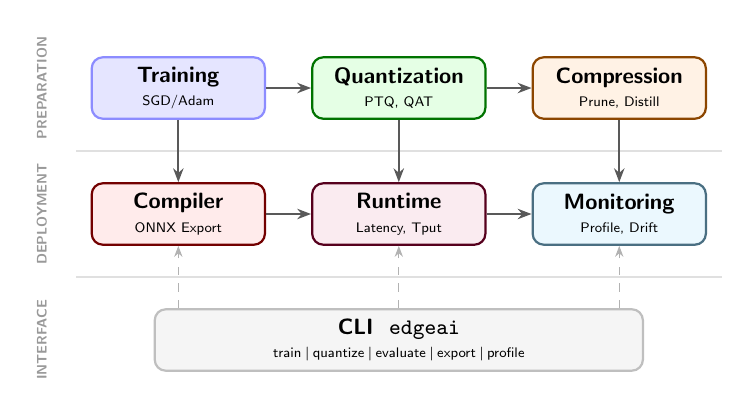
\begin{tikzpicture}[
    module/.style={draw, thick, rounded corners=4pt, minimum width=2.2cm,
                   minimum height=0.78cm, align=center, font=\footnotesize\sffamily},
    lbl/.style={font=\tiny\sffamily\bfseries, color=black!40, rotate=90, anchor=south},
    arr/.style={-{Stealth[length=5pt]}, thick, color=black!65},
    cliarr/.style={-{Stealth[length=4pt]}, color=black!30, dashed, thin},
    sep/.style={black!12, thick},
]

% ── Row 1: Model Preparation ──────────────────────────
\node[module, fill=blue!10, draw=blue!45] (train)
    at (0,0) {\textbf{Training}\\[-1pt]{\tiny SGD/Adam}};
\node[module, fill=green!10, draw=green!45!black] (quant)
    at (2.8,0) {\textbf{Quantization}\\[-1pt]{\tiny PTQ, QAT}};
\node[module, fill=orange!10, draw=orange!55!black] (comp)
    at (5.6,0) {\textbf{Compression}\\[-1pt]{\tiny Prune, Distill}};

% ── Row 2: Deployment ─────────────────────────────────
\node[module, fill=red!8, draw=red!45!black] (export)
    at (0,-1.6) {\textbf{Compiler}\\[-1pt]{\tiny ONNX Export}};
\node[module, fill=purple!8, draw=purple!45!black] (runtime)
    at (2.8,-1.6) {\textbf{Runtime}\\[-1pt]{\tiny Latency, Tput}};
\node[module, fill=cyan!8, draw=cyan!45!black] (monitor)
    at (5.6,-1.6) {\textbf{Monitoring}\\[-1pt]{\tiny Profile, Drift}};

% ── Row 3: CLI ────────────────────────────────────────
\node[module, fill=gray!8, draw=gray!50, minimum width=6.2cm] (cli)
    at (2.8,-3.2) {\textbf{CLI}~~\texttt{edgeai}\\[-1pt]{\tiny train\,$|$\,quantize\,$|$\,evaluate\,$|$\,export\,$|$\,profile}};

% ── Phase labels (left margin, rotated) ───────────────
\node[lbl] at (-1.55, 0)    {PREPARATION};
\node[lbl] at (-1.55,-1.6)  {DEPLOYMENT};
\node[lbl] at (-1.55,-3.2)  {INTERFACE};

% ── Separators ────────────────────────────────────────
\draw[sep] (-1.3,-0.8) -- (6.9,-0.8);
\draw[sep] (-1.3,-2.4) -- (6.9,-2.4);

% ── Row 1 data flow (horizontal) ─────────────────────
\draw[arr] (train.east) -- (quant.west);
\draw[arr] (quant.east) -- (comp.west);

% ── Row 1 → Row 2 (vertical, straight down) ──────────
\draw[arr] (train.south)  -- (export.north);
\draw[arr] (quant.south)  -- (runtime.north);
\draw[arr] (comp.south)   -- (monitor.north);

% ── Row 2 data flow (horizontal) ─────────────────────
\draw[arr] (export.east)   -- (runtime.west);
\draw[arr] (runtime.east)  -- (monitor.west);

% ── CLI dashed arrows (straight up to Row 2) ─────────
\draw[cliarr] (cli.north -| export)  -- (export.south);
\draw[cliarr] (cli.north -| runtime) -- (runtime.south);
\draw[cliarr] (cli.north -| monitor) -- (monitor.south);

\end{tikzpicture}
\caption{Malak software architecture. Solid arrows show data flow: horizontally within each layer and vertically from preparation to deployment. Dashed arrows indicate CLI access points.}
\label{fig:architecture}
\end{figure}

\subsection{Training Module}

The \texttt{Trainer} class provides a configurable training loop supporting SGD and Adam optimizers with cosine annealing scheduling.
Dataset loaders for CIFAR-10 and Fashion-MNIST include standard data augmentation (random crop, horizontal flip) and normalization.
The trainer automatically tracks the best model checkpoint and reports per-epoch accuracy and latency.

\subsection{Quantization Module}

The quantization module provides three classes:

\begin{itemize}
    \item \textbf{DynamicPTQ}: Wraps \texttt{torch.quantization.quantize\_dynamic} to quantize Linear layers to INT8. Requires no calibration data. Suitable for models dominated by fully-connected layers.
    \item \textbf{StaticPTQ}: Inserts observers, runs a calibration pass over a representative dataset, and converts all supported layers to INT8. Produces full model compression.
    \item \textbf{QAT}: A three-step API (\texttt{prepare} $\to$ \texttt{train} $\to$ \texttt{convert}) that inserts fake-quantization observers during training, allowing weights to adapt to quantization noise before final INT8 conversion.
\end{itemize}

The QAT workflow is illustrated below:

\noindent\fbox{\parbox{0.95\linewidth}{\small\texttt{%
from malak.quantization import QAT\\[2pt]
qat = QAT()\\
model = qat.prepare(model, backend="fbgemm")\\
model = qat.train(model, train\_loader,\\
\hspace*{2em}test\_loader, epochs=5)\\
quantized = qat.convert(model)
}}}

\subsection{Compression Module}

The compression module provides magnitude pruning (\texttt{MagnitudePruner}), structured filter pruning (\texttt{StructuredPruner}), and knowledge distillation (\texttt{KnowledgeDistiller}).
The pruners support configurable sparsity levels with \texttt{remove\_masks()} to make pruning permanent and \texttt{sparsity()} to report actual sparsity.
The distiller trains a student model using a weighted combination of cross-entropy (hard labels) and KL-divergence (temperature-scaled soft labels from the teacher), following~\cite{distillation}.

\subsection{Supporting Modules}

The \textbf{Compiler} module exports models to ONNX format with optional validation.
The \textbf{Runtime} module benchmarks inference latency and throughput.
The \textbf{Monitoring} module provides per-layer latency profiling via forward hooks and KL-divergence-based distribution drift detection for deployed models.
The \texttt{edgeai} CLI exposes all modules through subcommands (\texttt{train}, \texttt{quantize}, \texttt{evaluate}, \texttt{export}, \texttt{profile}).

%% ================================================================
\section{Experimental Validation}
\label{sec:experiments}
%% ================================================================

We validate Malak through four experiments covering quantization, architecture comparison, pruning, and cross-dataset evaluation.
All experiments use CPU inference (Intel Core i7) with PyTorch 2.x.
Results are stored as JSON files in the repository and every number reported is directly measured.
All experiments are reproducible via scripts in the \texttt{experiments/} directory.

\subsection{Experiment 1: MobileNetV2 Quantization}

We train MobileNetV2~\cite{mobilenetv3} (2.24M parameters, first convolution modified for 32$\times$32 input) on CIFAR-10 for 15 epochs with SGD (lr=0.01, momentum=0.9, cosine annealing).
We then apply dynamic PTQ and QAT (5 fine-tuning epochs with lr=0.001).
Table~\ref{tab:cifar10} shows the results.

\begin{table}[t]
\caption{MobileNetV2 quantization results on CIFAR-10.}
\label{tab:cifar10}
\centering
\begin{tabular}{lccc}
\toprule
\textbf{Method} & \textbf{Acc. (\%)} & \textbf{Size (MB)} & \textbf{Compr.} \\
\midrule
FP32 Baseline & 77.81 & 8.76 & 1.00$\times$ \\
Dynamic PTQ & 77.84 & 8.73 & 1.00$\times$ \\
QAT (INT8) & 76.72 & 2.82 & 3.10$\times$ \\
\bottomrule
\end{tabular}
\end{table}

Dynamic PTQ preserves accuracy (within 0.03\%) but provides minimal size reduction because it only quantizes Linear layers while the convolutional layers---which dominate MobileNetV2---remain in FP32.
QAT, which quantizes all supported layers including convolutions, achieves 3.10$\times$ compression with 1.09\% accuracy drop.

We note that the 77.81\% FP32 baseline is below published state-of-the-art for MobileNetV2 on CIFAR-10 ($\sim$94\%) due to our shortened training schedule (15 epochs vs.\ typical 200+ epochs with advanced augmentation).
The purpose of this experiment is to validate the toolkit's quantization pipeline, not to achieve maximum accuracy.
The relative compression ratios and accuracy drops are consistent with published quantization studies~\cite{ptq, qat}.

\subsection{Experiment 2: Architecture Comparison}

We compare ResNet18 (11.2M parameters) and EfficientNet-B0~\cite{efficientnet} (4.0M parameters) on CIFAR-10, training each for 15 epochs with SGD and applying dynamic INT8 PTQ.
Table~\ref{tab:arch} shows the results.

\begin{table}[t]
\caption{Architecture comparison with dynamic INT8 PTQ on CIFAR-10.}
\label{tab:arch}
\centering
\begin{tabular}{lcccc}
\toprule
\textbf{Model} & \textbf{FP32} & \textbf{INT8} & \textbf{Drop} & \textbf{Compr.} \\
\midrule
ResNet18 & 87.41\% & 87.38\% & 0.03\% & 1.00$\times$ \\
EfficientNet-B0 & 66.81\% & 66.68\% & 0.13\% & 1.00$\times$ \\
\bottomrule
\end{tabular}
\end{table}

Dynamic PTQ preserves accuracy within 0.13\% for both architectures.
The 1.00$\times$ compression ratio is expected: dynamic PTQ only quantizes \texttt{nn.Linear} layers at runtime, and both architectures are dominated by convolutional layers whose weights remain in FP32.
The EfficientNet-B0 baseline accuracy (66.81\%) is lower than ResNet18 (87.41\%) because EfficientNet's compound scaling was designed for 224$\times$224 ImageNet inputs and requires longer training schedules to converge on 32$\times$32 CIFAR-10 images.

\subsection{Experiment 3: Pruning}

We apply L1-unstructured magnitude pruning at 30\%, 50\%, and 70\% target sparsity to a trained MobileNetV2, followed by 3 epochs of fine-tuning per sparsity level.
We also test L2-structured filter pruning at 30\% and 50\% sparsity.
Table~\ref{tab:pruning} shows the results.

\begin{table}[t]
\caption{Pruning results on CIFAR-10 MobileNetV2 (with fine-tuning).}
\label{tab:pruning}
\centering
\begin{tabular}{llccc}
\toprule
\textbf{Method} & \textbf{Target} & \textbf{Acc. (\%)} & \textbf{Drop} & \textbf{Actual} \\
\midrule
Baseline & 0\% & 77.81 & --- & 0\% \\
\midrule
Magnitude & 30\% & 77.32 & 0.49\% & 29.5\% \\
Magnitude & 50\% & 75.66 & 2.15\% & 49.2\% \\
Magnitude & 70\% & 70.47 & 7.34\% & 68.9\% \\
\midrule
Structured & 30\% & 72.86 & 4.95\% & 29.6\% \\
Structured & 50\% & 64.17 & 13.64\% & 49.2\% \\
\bottomrule
\end{tabular}
\end{table}

Magnitude pruning at 30\% sparsity causes negligible accuracy loss (0.49\%), while 50\% sparsity results in a moderate 2.15\% drop.
At 70\% sparsity, accuracy drops by 7.34\%, indicating that more aggressive fine-tuning (e.g., 10--20 epochs) would be beneficial at high sparsity levels.
Structured pruning causes larger accuracy drops than magnitude pruning at the same sparsity level because removing entire filters is more destructive than zeroing individual weights.
This is consistent with findings in the pruning literature~\cite{structured-pruning, lottery-ticket}.

\subsection{Experiment 4: Fashion-MNIST with SimpleCNN}

We train a custom SimpleCNN (458K parameters: three convolutional layers with max-pooling, followed by two fully-connected layers) on Fashion-MNIST for 20 epochs with Adam (lr=0.001) and apply dynamic INT8 PTQ.
Table~\ref{tab:fmnist} shows the results.

\begin{table}[t]
\caption{SimpleCNN results on Fashion-MNIST with dynamic PTQ.}
\label{tab:fmnist}
\centering
\begin{tabular}{lccc}
\toprule
\textbf{Method} & \textbf{Acc. (\%)} & \textbf{Size (MB)} & \textbf{Compr.} \\
\midrule
FP32 Baseline & 92.19 & 1.75 & 1.00$\times$ \\
Dynamic PTQ & 92.20 & 0.60 & 2.91$\times$ \\
\bottomrule
\end{tabular}
\end{table}

Unlike the convolutional-heavy architectures in Experiments 1--2, SimpleCNN has substantial fully-connected layers (64$\times$7$\times$7 $\to$ 128 $\to$ 10), which are quantized by dynamic PTQ.
This results in 2.91$\times$ compression with no accuracy loss, demonstrating that dynamic PTQ is effective for FC-heavy models.
The 92.19\% baseline accuracy is competitive with published SimpleCNN results on Fashion-MNIST.

\subsection{Embedded Proof-of-Concept}

The repository includes a C implementation of SimpleCNN inference using INT8 weights exported by a Python script.
The C code implements naive conv2d, maxpool, fully-connected, and ReLU operations with symmetric INT8 quantization, targeting ARM Cortex-M7 (STM32H7) via \texttt{arm-none-eabi-gcc}.
This implementation serves as a proof-of-concept for the export pipeline; production-quality embedded inference would require optimized kernels from CMSIS-NN~\cite{cmsis-nn} or TFLite Micro~\cite{tflitemicro}.

%% ================================================================
\section{Discussion}
\label{sec:discussion}
%% ================================================================

\subsection{Key Findings}

The experimental results demonstrate three findings:
(1)~QAT is the most effective quantization method for convolutional models, achieving 3.10$\times$ compression with minimal accuracy loss, while dynamic PTQ provides negligible compression for conv-heavy architectures but is effective for FC-heavy models (2.91$\times$ on SimpleCNN).
(2)~Magnitude pruning is more accuracy-preserving than structured pruning at the same sparsity level, at the cost of requiring sparse matrix support for inference speedup.
(3)~The Malak API successfully produces reproducible, measurable results across four architectures and two datasets, validating its correctness.

\subsection{Limitations}

This work has several limitations that should be acknowledged:

\begin{enumerate}
    \item \textbf{Limited baselines.} Our FP32 accuracies (77.81\% MobileNetV2, 66.81\% EfficientNet-B0) are below published state-of-the-art due to abbreviated training schedules. While the relative compression metrics remain valid, results at higher baselines may differ.
    \item \textbf{Single-run results.} All experiments report single-run results without standard deviations. Stochastic training introduces variance that is not captured.
    \item \textbf{CPU-only evaluation.} All latency measurements are on desktop CPU, not on actual edge hardware. Inference speedup from quantization depends heavily on hardware support for INT8 operations.
    \item \textbf{Limited scope.} The toolkit supports only CIFAR-10 and Fashion-MNIST datasets and a small set of architectures. Extension to larger datasets (ImageNet) and domain-specific tasks is left to users.
    \item \textbf{Wrapper-level contribution.} Malak wraps existing PyTorch APIs rather than introducing new algorithms. Its value lies in usability and reproducibility, not algorithmic novelty.
    \item \textbf{Embedded deployment.} The C inference code is a proof-of-concept with floating-point accumulation, not a production-ready embedded runtime.
\end{enumerate}

\subsection{Comparison with Existing Tools}

Malak's primary advantage over raw PyTorch is reduced boilerplate: the QAT workflow requires 5 lines of code (the code example in Section~\ref{sec:architecture}) compared to $\sim$40 lines using PyTorch directly.
Compared to Intel Neural Compressor~\cite{intel-nc}, Malak is simpler to install (pure Python, no hardware-specific dependencies) but offers fewer quantization strategies and no hardware-aware optimization.
Compared to TFLite, Malak stays within the PyTorch ecosystem but lacks a production-quality embedded runtime.
Malak is best suited for rapid prototyping and educational use rather than production deployment.

%% ================================================================
\section{Conclusions}
\label{sec:conclusion}
%% ================================================================

We presented Malak, an open-source Python toolkit for edge AI model optimization that provides a unified API for quantization, pruning, distillation, ONNX export, profiling, and drift detection.
Validation across four experiments on CIFAR-10 and Fashion-MNIST demonstrates that the toolkit produces correct and reproducible compression results.
QAT achieves 3.10$\times$ compression with 1.09\% accuracy drop on MobileNetV2, while magnitude pruning at 50\% sparsity retains accuracy within 2.15\% of the baseline.

Future work includes:
(1)~integration with CMSIS-NN for production-quality embedded inference,
(2)~support for mixed-precision quantization~\cite{mixed-precision},
(3)~multi-run experiments with statistical reporting,
(4)~extending the training pipeline to ImageNet-scale datasets, and
(5)~automated compression policy search combining quantization and pruning.

The toolkit is available at \url{https://github.com/alnemari-m/malak-platform} under the MIT license.

\section*{Acknowledgments}
The author thanks the open-source PyTorch community for the quantization and pruning APIs upon which Malak is built.

\vspace{6pt}
\noindent\textbf{Mohammed Hassan Alnemari} received the B.Sc.\ degree in computer engineering from Taif University, Saudi Arabia, and the M.S.\ and Ph.D.\ degrees in computer engineering from the University of California, Irvine (UCI), USA. He is currently an Assistant Professor and Chair of the Computer Engineering Department at the University of Tabuk, Saudi Arabia. His research interests include Edge Artificial Intelligence (Edge AI), TinyML, neural network compression, efficient deep learning architectures, and hardware--software co-design for intelligent embedded systems. His work focuses on enabling energy-efficient machine learning inference on resource-constrained edge devices.

\begin{thebibliography}{99}

\bibitem{warden2019tinyml}
P.~Warden and D.~Situnayake, \textit{TinyML: Machine Learning with TensorFlow Lite on Arduino and Ultra-Low-Power Microcontrollers}. O'Reilly Media, 2019.

\bibitem{edge-ai-survey}
Z.~Zhou, X.~Chen, E.~Li, L.~Zeng, K.~Luo, and J.~Zhang, ``Edge intelligence: The confluence of edge computing and artificial intelligence,'' \textit{IEEE Internet of Things Journal}, vol.~7, no.~8, pp.~7457--7469, 2020.

\bibitem{ptq}
B.~Jacob \textit{et al.}, ``Quantization and training of neural networks for efficient integer-arithmetic-only inference,'' in \textit{Proc. IEEE CVPR}, 2018, pp.~2704--2713.

\bibitem{qat}
Y.~Bhalgat, J.~Lee, M.~Nagel, T.~Blankevoort, and N.~Kwak, ``Quantization aware training for low bit-width neural networks,'' in \textit{NeurIPS Workshop}, 2020.

\bibitem{tflite}
M.~Abadi \textit{et al.}, ``TensorFlow Lite: On-device machine learning framework,'' Google Research, 2019.

\bibitem{tflitemicro}
R.~David \textit{et al.}, ``TensorFlow Lite Micro: Embedded machine learning for TinyML systems,'' in \textit{Proc. MLSys}, vol.~3, 2021, pp.~800--811.

\bibitem{tvm}
T.~Chen \textit{et al.}, ``TVM: An automated end-to-end optimizing compiler for deep learning,'' in \textit{Proc. USENIX OSDI}, 2018, pp.~578--594.

\bibitem{cmsis-nn}
L.~Lai, N.~Suda, and V.~Chandra, ``CMSIS-NN: Efficient neural network kernels for Arm Cortex-M CPUs,'' \textit{arXiv preprint arXiv:1801.06601}, 2018.

\bibitem{intel-nc}
Intel Corporation, ``Intel Neural Compressor: An open-source Python library for model compression,'' GitHub repository, 2021.

\bibitem{model-compression-survey}
L.~Deng, G.~Li, S.~Han, L.~Shi, and Y.~Xie, ``Model compression and hardware acceleration for neural networks: A comprehensive survey,'' \textit{Proc. IEEE}, vol.~108, no.~4, pp.~485--532, 2020.

\bibitem{distillation}
G.~Hinton, O.~Vinyals, and J.~Dean, ``Distilling the knowledge in a neural network,'' in \textit{NIPS Deep Learning Workshop}, 2015.

\bibitem{structured-pruning}
Z.~Liu \textit{et al.}, ``Learning efficient convolutional networks through network slimming,'' in \textit{Proc. IEEE ICCV}, 2017, pp.~2736--2744.

\bibitem{lottery-ticket}
J.~Frankle and M.~Carlin, ``The lottery ticket hypothesis: Finding sparse, trainable neural networks,'' \textit{arXiv preprint arXiv:1803.03635}, 2018.

\bibitem{mobilenetv3}
A.~Howard \textit{et al.}, ``Searching for MobileNetV3,'' in \textit{Proc. IEEE ICCV}, 2019, pp.~1314--1324.

\bibitem{efficientnet}
M.~Tan and Q.~Le, ``EfficientNet: Rethinking model scaling for convolutional neural networks,'' in \textit{Proc. ICML}, 2019, pp.~6105--6114.

\bibitem{mixed-precision}
K.~Wang, Z.~Liu, Y.~Lin, J.~Lin, and S.~Han, ``HAQ: Hardware-aware automated quantization with mixed precision,'' in \textit{Proc. IEEE CVPR}, 2019, pp.~8612--8620.

\bibitem{onnx}
J.~Bai, F.~Lu, K.~Zhang \textit{et al.}, ``ONNX: Open neural network exchange,'' GitHub repository, 2019.

\end{thebibliography}

\end{document}
